\documentclass{beamer}
\input{../utils/preamble}
\createdgmtitle{3}

%--------------------------------------------------------------------------------
\begin{document}
%--------------------------------------------------------------------------------
\begin{frame}[noframenumbering,plain]
	\titlepage
	\resetonslide
\end{frame}
%=======
\begin{frame}{Recap of Previous Lecture}
    \begin{block}{Jacobian Matrix}
		Let $\bff: \bbR^m \rightarrow \bbR^m$ be a differentiable function.
		\[
			\bz = \bff(\bx), \quad 
			\bJ =  \frac{\partial \bz}{\partial \bx} =
			\begin{pmatrix}
				\frac{\partial z_1}{\partial x_1} & \dots & \frac{\partial z_1}{\partial x_m} \\
				\vdots & \ddots & \vdots \\ 
				\frac{\partial z_m}{\partial x_1} & \dots & \frac{\partial z_m}{\partial x_m}
			\end{pmatrix} \in \bbR^{m \times m}
		\]
		\vspace{-0.3cm}
	\end{block}
	\begin{block}{Change of Variables Theorem (CoV)}
		Let $\bx\in \bbR^m$ be a random vector with density $p(\bx)$, and let $\bff: \bbR^m \rightarrow \bbR^m$ be a $C^1$-diffeomorphism ($\bff$ and $\bff^{-1}$ are continuously differentiable mappings). 
		If $\bz = \bff(\bx)$, then
		\begin{align*}
			p(\bx) &= p(\bz) |\det(\bJ_{\bff})| = p(\bz) \left|\det \left( \frac{\partial \bz}{\partial \bx} \right) \right| 
			= p(\bff(\bx)) \left|\det \left(  \frac{\partial \bff(\bx)}{\partial \bx} \right) \right| \\
			p(\bz) &= p(\bx) |\det(\bJ_{\bff^{-1}})| = p(\bx) \left|\det \left(  \frac{\partial \bx}{\partial \bz} \right) \right| 
			= p(\bff^{-1}(\bz)) \left|\det \left(  \frac{\partial \bff^{-1}(\bz)}{\partial \bz} \right) \right|
		\end{align*}
		\vspace{-0.5cm}
	\end{block}
\end{frame}
%=======
\begin{frame}{Recap of Previous Lecture}
    \myfootnotewithlink{https://arxiv.org/abs/1605.08803}{Dinh L., Sohl-Dickstein J., Bengio S. Density Estimation Using Real NVP, 2016} 
	\begin{block}{Definition}
		A normalizing flow is a $C^1$-diffeomorphism that transforms data $\bx$ to noise $\bz$.
	\end{block}
	\vspace{-0.1cm}
	\begin{figure}
		\includegraphics[width=0.85\linewidth]{figs/flows_how2}
	\end{figure}
	\vspace{-0.5cm}
	\begin{block}{Log-Likelihood}
		\vspace{-0.5cm}
		\[
			\log \pt(\bx) = \log p(\bff_K \circ \cdots \circ \bff_1(\bx)) + \sum_{k=1}^K\log |\det (\bJ_{\bff_k})|
		\]
	\end{block}
\end{frame}
%=======
\begin{frame}{Recap of Previous Lecture}
    \myfootnote{\href{https://arxiv.org/abs/1807.03039}{Kingma D. P., et al. Glow: Generative Flow With Invertible 1x1 Convolutions, 2018}  \\
	\href{https://arxiv.org/abs/1901.11137}{Hoogeboom E., et al. Emerging Convolutions for Generative Normalizing Flows, 2019}
	}
	\vspace{-0.5cm}
	\begin{block}{Flow Log-Likelihood}
		\vspace{-0.3cm}
		\[
			\log \pt(\bx) = \log p(\bff_{\btheta}(\bx)) + \log |\det (\bJ_\bff)|
		\]
		\vspace{-0.5cm}
	\end{block}
	One significant challenge is efficiently computing the Jacobian determinant.
	\begin{block}{Linear Flows}	
		\vspace{-0.2cm}
		\[
			\bz = \bff_{\btheta}(\bx) = \bW \bx, \quad \bW \in \bbR^{m \times m}, \quad \btheta = \bW, \quad \bJ_\bff = \bW^T
		\]
	\end{block}
	\vspace{-0.3cm}
	\begin{itemize}
		\item LU Decomposition:
		\[
			\bW = \bP \bL \bU.
		\]
		\item QR Decomposition:
		\[
			\bW = \bQ \bR.
		\]
	\end{itemize}
	Decomposition is performed only once during initialization. Then the decomposed matrices ($\bP, \bL, \bU$ or $\bQ, \bR$) are optimized.
\end{frame}
%=======
\begin{frame}{Recap of Previous Lecture}
    \myfootnotewithlink{https://arxiv.org/abs/1705.07057}{Papamakarios G., Pavlakou T., Murray I. Masked Autoregressive Flow for Density Estimation, 2017} 
	Consider an autoregressive model:
	\vspace{-0.3cm}
	{\small
		\[
		\pt(\bx) = \prod_{j=1}^m \pt(x_j | \bx_{1:j - 1}), \quad
		\pt(x_j | \bx_{1:j - 1}) = \cN \left(\mu_{j, \btheta}(\bx_{1:j-1}), \sigma^2_{j, \btheta} (\bx_{1:j-1})\right).
		\]
	}
	\vspace{-0.5cm}
	\begin{block}{Gaussian Autoregressive Normalizing Flow}
		\vspace{-0.5cm}
		\begin{align*}
			\bx &= \bff^{-1}_{\btheta}(\bz) \quad \Rightarrow \quad {\color{violet} x_j} = \sigma_{j, \btheta} ({\color{violet} \bx_{1:j-1}}) \cdot {\color{teal} z_j} + \mu_{j, \btheta}({\color{violet} \bx_{1:j-1}}). \\
			\bz &= \bff_{\btheta}(\bx) \quad \Rightarrow \quad {\color{teal} z_j} = \left({\color{violet}x_j} - \mu_{j, \btheta}({\color{violet}\bx_{1:j-1}}) \right) \cdot \frac{1}{ \sigma_{j, \btheta} ({\color{violet}\bx_{1:j-1}})}.
		\end{align*}
		\vspace{-0.5cm}
	\end{block}
	\begin{itemize}
		\item This transformation is both \textbf{$C^1$-diffeomorphism}, mapping $p(\bz)$ to $\pt(\bx)$.
		\item The Jacobian matrix for this transformation is triangular.
	\end{itemize}
	The generative function $\bff^{-1}_{\btheta}(\bz)$ is \textbf{sequential}, while the inference function $\bff_{\btheta}(\bx)$ is \textbf{not sequential}.
\end{frame}
%=======
\begin{frame}{Recap of Previous Lecture}
    \myfootnotewithlink{https://arxiv.org/abs/1605.08803}{Dinh L., Sohl-Dickstein J., Bengio S. Density Estimation Using Real NVP, 2016} 

	Let us partition $\bx$ and $\bz$ into two groups: 
	\[
		\bx = [\bx_1, \bx_2] = [\bx_{1:d}, \bx_{d+1:m}]; \quad \bz = [\bz_1, \bz_2] = [\bz_{1:d}, \bz_{d+1:m}].
	\]
	\vspace{-0.7cm}
	\begin{block}{Coupling Layer}
		\vspace{-0.7cm}
		\[
			\begin{cases} {\color{violet}\bx_1} = {\color{teal}\bz_1}; \\ {\color{violet}\bx_2} = {\color{teal}\bz_2} \odot \bsigma_{\btheta}({\color{teal}\bz_1}) + \bmu_{\btheta}({\color{teal}\bz_1}).\end{cases}  
			\begin{cases} {\color{teal}\bz_1} ={\color{violet} \bx_1}; \\ {\color{teal}\bz_2} = \left({\color{violet}\bx_2} - \bmu_{\btheta}({\color{violet}\bx_1}) \right) \odot \frac{1}{\bsigma_{\btheta}({\color{violet}\bx_1})}.\end{cases}
		\]
		Both density estimation and sampling require just a single pass!
	\end{block}
	\begin{block}{Jacobian}
		\vspace{-0.3cm}
		\[
			\det \left( \frac{\partial \bz}{\partial \bx} \right) = \det 
			\begin{pmatrix}
				\bI_d & 0_{d \times (m - d)} \\
				\frac{\partial \bz_2}{\partial \bx_1} & \frac{\partial \bz_2}{\partial \bx_2}
			\end{pmatrix} = \prod_{j=1}^{m - d} \frac{1}{\sigma_{j, \btheta}(\bx_1)}.
		\]
	\end{block}
	A coupling layer is a special instance of an gaussian autoregressive normalizing flow.
\end{frame}
%=======
\begin{frame}{Recap of Previous Lecture}
	\begin{block}{Posterior Distribution (Bayes' Theorem)}
		\[
			p(\btheta | \bx) = \frac{p(\bx | \btheta) p(\btheta)}{p(\bx)} = \frac{p(\bx | \btheta) p(\btheta)}{\int p(\bx | \btheta) p(\btheta) d \btheta} 
		\]
		\begin{itemize}
			\item $\bx$ -- observed variables;
			\item $\btheta$ -- unobserved variables (latent parameters);
			\item $\pt(\bx) = p(\bx | \btheta)$ -- likelihood;
			\item $p(\bx) = \int p(\bx | \btheta) p(\btheta) d \btheta$ -- evidence;
			\item $p(\btheta)$ -- prior distribution;
			\item $p(\btheta | \bx)$ -- posterior distribution.
		\end{itemize}
	\end{block}
\end{frame}
%=======
\begin{frame}{Outline}
    \tableofcontents
\end{frame}
%=======
\section{Latent Variable Models (LVM) (continued)}
%=======
\begin{frame}{Latent Variable Models (LVM)}
	\begin{block}{Maximum Likelihood Extimation (MLE) Problem}
		\vspace{-0.7cm}
		\[
			\btheta^* = \argmax_{\btheta} \pt(\bX) = \argmax_{\btheta} \prod_{i=1}^n \pt(\bx_i) = \argmax_{\btheta} \sum_{i=1}^n \log \pt(\bx_i).
		\]
		\vspace{-0.5cm}
	\end{block}
    \eqpause
	The distribution $\pt(\bx)$ can be highly complex and often intractable (just like the true data distribution $\pd(\bx)$).
    \eqpause
	\begin{block}{Extended Probabilistic Model}
		Introduce a latent variable $\bz$ for each observed sample $\bx$:
		\[
			\pt(\bx, \bz) = \pt(\bx | \bz) p(\bz); \quad 
		\log \pt(\bx, \bz) = \log \pt(\bx | \bz) + \log p(\bz).
		\]
		\[
			\nextonslide{\pt(\bx) = \int \pt(\bx, \bz) d\bz = \int \pt(\bx | \bz) p(\bz) d\bz.}
		\]
	\end{block}
    \eqpause
	\vspace{-0.3cm}
	\begin{block}{Motivation}
		Both $\pt(\bx | \bz)$ and $p(\bz)$ are usually much simpler than $\pt(\bx)$.
	\end{block}
\end{frame}
%=======
\begin{frame}{Latent Variable Models (LVM)}
    \myfootnote{Bishop\,C. Pattern Recognition and Machine Learning, 2006}
	\[
		\log \pt(\bx) = \log \int \pt(\bx | \bz) p(\bz) d\bz \rightarrow \max_{\btheta}
	\]
    \eqpause
	\vspace{-0.6cm}
	\begin{block}{Examples}
		\begin{minipage}[t]{0.45\columnwidth}
			\textit{Mixture of Gaussians} \\
			\vspace{-0.5cm}
			\begin{figure}
				\centering
				\includegraphics[width=0.75\linewidth]{figs/mixture_of_gaussians}
			\end{figure}
			\vspace{-0.5cm}
			\begin{itemize}
				\item $\pt(\bx | z) = \cN(\bmu_z, \bSigma_z)$
				\item $p(z) = \Cat(\bpi)$
			\end{itemize}
		\end{minipage}%
        \eqpause
		\begin{minipage}[t]{0.53\columnwidth}
			\textit{PCA Model} \\
			\vspace{-0.5cm}
			\begin{figure}
				\centering
				\includegraphics[width=.7\linewidth]{figs/pca}
			\end{figure}
			\vspace{-0.3cm}
			\begin{itemize}
				\item $\pt(\bx | \bz) = \cN(\bW \bz + \bmu, \sigma^2 \bI)$
				\item $p(\bz) = \cN(0, \bI)$
			\end{itemize}
		\end{minipage}
	\end{block}
\end{frame}
%=======
\begin{frame}{MLE for LVM}
    \myfootnotewithlink{https://jmtomczak.github.io/blog/4/4\_VAE.html}{image credit: https://jmtomczak.github.io/blog/4/4\_VAE.html}
	\[
		\sum_{i=1}^n \log \pt(\bx_i) = \sum_{i=1}^n \log \int \pt(\bx_i| \bz_i) p(\bz_i) d\bz_i \rightarrow \max_{\btheta}.
	\]
    \eqpause
	\vspace{-0.6cm}
	\begin{figure}
		\includegraphics[width=.65\linewidth]{figs/lvm_diagram}
	\end{figure}
    \eqpause
	\vspace{-0.5cm}
	\begin{block}{Naive Monte Carlo Estimation}
		\vspace{-0.7cm}
		\[
			\log \pt(\bx) = \log \bbE_{p(\bz)} \pt(\bx | \bz) \geq \bbE_{p(\bz)} \log \pt(\bx | \bz) \approx \frac{1}{K} \sum_{k=1}^{K} \log \pt(\bx | \bz_k),
		\]
		\vspace{-0.7cm} \\
		where $\bz_k \sim p(\bz)$. \\
        \eqpause
		\textbf{Challenge:} As the dimensionality of $\bz$ increases, the number of samples needed to adequately cover the latent space grows exponentially.
	\end{block}
\end{frame}
%=======
\section{Variational Evidence Lower Bound (ELBO)}
%=======
\begin{frame}{ELBO Derivation I}
	\begin{block}{Inequality Derivation}
		\vspace{-0.7cm}
		\begin{multline*}
			\log \pt(\bx) 
			= \log \int \pt(\bx, \bz) d\bz 
			\nextonslide{= \log \int \frac{q(\bz)}{q(\bz)} \pt(\bx, \bz) d\bz}
			\nextonslide{= \\ = \log \bbE_{q} \left[\frac{\pt(\bx, \bz)}{q(\bz)} \right]}
			\nextonslide{ \geq \bbE_{q} \log \frac{\pt(\bx, \bz)}{q(\bz)} = \cL_{q, \btheta}(\bx)}
		\end{multline*}
		\vspace{-0.3cm}
	\end{block}
    \eqpause
	\begin{itemize}
		\item Here, $q(\bz)$ is any distribution such that $\int q(\bz) d\bz = 1$.
		\item {\color{gray} We assume that $\text{supp}(q(\bz)) = \text{supp}(\pt(\bz | \bx)) = \bbR^{d}$}.
	\end{itemize}
    \eqpause
	\begin{block}{Variational Evidence Lower Bound (ELBO)}
		\[
			 \cL_{q, \btheta}(\bx) = \bbE_{q} \log \frac{\pt(\bx, \bz)}{q(\bz)}  \leq \log \pt(\bx) 
		\]
    	\eqpause
		This inequality holds for any choice of $q(\bz)$.
	\end{block}
\end{frame}
%=======
\begin{frame}{ELBO Derivation II}
	\vspace{-0.3cm}
	\[
		{\color{teal}\pt(\bz|\bx) = \frac{\pt(\bx, \bz)}{\pt(\bx)}}
	\]
	\vspace{-0.4cm}
	\begin{block}{Equality Derivation}
		\vspace{-0.7cm}
		\begin{multline*}
			\cL_{q, \btheta}(\bx) = \int q(\bz) \log \frac{\color{teal}\pt(\bx, \bz)}{q(\bz)}d\bz 
			\nextonslide{= \\ = \int q(\bz) \log \frac{\color{teal}\pt(\bz|\bx)\pt(\bx)}{q(\bz)}d\bz}
			\nextonslide{ = \\ = \int q(\bz) \log \pt(\bx) d\bz + \int q(\bz) \log \frac{\pt(\bz|\bx)}{q(\bz)}d\bz}
			\nextonslide{ = \\ = \log \pt(\bx) - \KL(q(\bz) \| \pt(\bz|\bx))}
		\end{multline*}
	\end{block}
    \eqpause
	\vspace{-0.7cm}
	\begin{block}{Variational Decomposition}
		\vspace{-0.2cm}
		\[
			\log \pt(\bx) = \cL_{q, \btheta}(\bx) + {\color{violet}\KL(q(\bz) \| \pt(\bz|\bx))} \geq \cL_{q, \btheta}(\bx).
		\]
	\end{block}
    \eqpause
	Here, ${\color{violet}\KL(q(\bz) \| \pt(\bz|\bx)) \geq 0}$.
\end{frame}
%=======
\begin{frame}{Variational Evidence Lower Bound (ELBO)}
	\vspace{-0.3cm}
	\begin{align*}
		\cL_{q, \btheta}(\bx) &= \int q(\bz) \log \frac{\color{violet}\pt(\bx, \bz)}{\color{teal}q(\bz)}d\bz \\ 
		\nextonslide{&= \int q(\bz) \log {\color{violet}\pt(\bx | \bz)} d\bz + \int q(\bz) \log \frac{\color{violet}p(\bz)}{\color{teal}q(\bz)}d\bz} \\ 
		\nextonslide{&= \bbE_{q} \log \pt(\bx | \bz) - \KL (q(\bz) \| p(\bz))}
	\end{align*}
    \eqpause
	\vspace{-0.5cm}
	\begin{block}{Log-Likelihood Decomposition}
		\vspace{-0.8cm}
		\begin{multline*}
			\log \pt(\bx) = {\color{olive}\cL_{q, \btheta}(\bx)} + \KL(q(\bz) \| \pt(\bz|\bx)) 
			\nextonslide{ = \\ = {\color{olive}\bbE_{q} \log \pt(\bx | \bz) - \KL (q(\bz) \| p(\bz))} + \KL(q(\bz) \| \pt(\bz|\bx)).}
		\end{multline*}
		\vspace{-0.7cm}
	\end{block}
    \eqpause
	\begin{itemize}
		\item Instead of maximizing the likelihood, maximize the ELBO:
		\[
		\max_{\btheta} \pt(\bx) \quad \rightarrow \quad \max_{q, \btheta} \cL_{q, \btheta}(\bx)
		\]
        \eqpause
		\vspace{-0.3cm}
		\item Maximizing the ELBO with respect to the \textbf{variational} distribution $q$ is equivalent to minimizing the KL divergence:
		\[
		\argmax_q \cL_{q, \btheta}(\bx) \equiv \argmin_q \KL(q(\bz) \| \pt(\bz|\bx)).
		\]
	\end{itemize}
\end{frame}
%=======
\begin{frame}{Variational Posterior}
    \myfootnote{Bishop\,C. Pattern Recognition and Machine Learning, 2006}
	\[
		\cL_{q, \btheta}(\bx)  =  \bbE_{q} \log \pt(\bx | \bz) - \KL (q(\bz) \| p(\bz)) \rightarrow \max_{q, \btheta}.
	\]
	What is the optimal distribution $q^*(\bz)$ given fixed $\btheta^*$?
    \eqpause
	\vspace{-0.3cm}
	\begin{multline*}
		q^*(\bz) = \argmax_q \cL_{q, \btheta^*}(\bx) = \\
		= \argmin_q \KL(q(\bz) \| p_{\btheta^*}(\bz | \bx)) = p_{\btheta^*}(\bz| \bx).
	\end{multline*}
	\vspace{-0.3cm} \\
	Here we got the intuition about $q(\bz)$ – it estimates the posterior~$p_{\btheta^*}(\bz| \bx)$.
	\vspace{-0.3cm}
    \eqpause
	\begin{minipage}[t]{0.45\columnwidth}
		\begin{figure}
			\includegraphics[width=0.9\linewidth]{figs/em_bishop1}
		\end{figure}
	\end{minipage}%
	\begin{minipage}[t]{0.55\columnwidth}
		\begin{figure}
			\includegraphics[width=0.85\linewidth]{figs/em_bishop2}
		\end{figure}
	\end{minipage}
\end{frame}
%=======
\section{Amortized Inference}
%=======
\begin{frame}{Parametric Variable Posterior}
	\begin{block}{Variational Posterior}
		\vspace{-0.3cm}
		\[
			q(\bz) = \argmax_q \cL_{q, \btheta^*}(\bx) = \argmin_q \KL(q \| p) =
		p_{\btheta^*}(\bz| \bx).
		\]
		\eqpause
		\begin{itemize}
			\item {\color{violet}$p_{\btheta^*}(\bz| \bx)$ may be \textbf{intractable}};
			\item {\color{teal}$q(\bz)$ is individual for each data point $\bx$}.
		\end{itemize}
	\end{block}
	\eqpause
	\begin{block}{Amortized Variational Inference}
		We restrict the family of possible distributions $q(\bz)$ to a parametric class $q_{\bphi}(\bz| \bx)$, {\color{teal}conditioned on data $\bx$} and {\color{violet}parameterized by $\bphi$}.
	\end{block}		
	\eqpause
	\begin{block}{Gradient Update}
		\[
			\begin{bmatrix}
				\bphi_k \\
				\btheta_k
			\end{bmatrix}
			= \left.
			\begin{bmatrix}
				\bphi_{k-1} + \eta \cdot \nabla_{\bphi} \cL_{\bphi, \btheta}(\bx) \\
				\btheta_{k-1} + \eta \cdot \nabla_{\btheta} \cL_{\bphi, \btheta}(\bx)
			\end{bmatrix}
			\right|_{(\bphi_{k-1}, \btheta_{k-1})}
		\]
	\end{block}
\end{frame}
%=======
\begin{frame}{ELBO optimization}
	\myfootnote{Bishop C., Deep Learning: Foundations and Concepts, 2024}
	\begin{block}{Gradient Update}
		\[
			\begin{bmatrix}
				\bphi_k \\
				\btheta_k
			\end{bmatrix}
			= \left.
			\begin{bmatrix}
				\bphi_{k-1} + \eta \cdot \nabla_{\bphi} \cL_{\bphi, \btheta}(\bx) \\
				\btheta_{k-1} + \eta \cdot \nabla_{\btheta} \cL_{\bphi, \btheta}(\bx)
			\end{bmatrix}
			\right|_{(\bphi_{k-1}, \btheta_{k-1})}
		\]
	\end{block}
	\begin{figure}
		\includegraphics[width=\linewidth]{figs/em_bishop4}
	\end{figure}
		
\end{frame}
%=======
\begin{frame}{ELBO optimization}
	\begin{block}{ELBO}
		\vspace{-0.3cm}
		\[
			\log \pt(\bx) = \cL_{\bphi, \btheta}(\bx) + \KL(q_{\bphi}(\bz| \bx) \| \pt(\bz|\bx)) \geq \cL_{\bphi, \btheta}(\bx).
		\]
		\[
		 	\cL_{q, \btheta}(\bx) = \bbE_{q} \log \pt(\bx | \bz) - \KL(q_{\bphi}(\bz| \bx) \| p(\bz))
		\]
		\vspace{-0.5cm}
	\end{block}
	\eqpause
	\begin{block}{Gradient Update}
		\[
			\begin{bmatrix}
				\bphi_k \\
				\btheta_k
			\end{bmatrix}
			= \left.
			\begin{bmatrix}
				\bphi_{k-1} + \eta \cdot \nabla_{\bphi} \cL_{\bphi, \btheta}(\bx) \\
				\btheta_{k-1} + \eta \cdot \nabla_{\btheta} \cL_{\bphi, \btheta}(\bx)
			\end{bmatrix}
			\right|_{(\bphi_{k-1}, \btheta_{k-1})}
		\]
		\begin{itemize}
			\item $\bphi$ denotes the parameters of the variational posterior $q_{\bphi}(\bz| \bx)$.
			\item $\btheta$ represents the parameters of the generative model $\pt(\bx | \bz)$.
		\end{itemize}
	\end{block}
	\eqpause
	The remaining step is to obtain \textbf{unbiased} Monte Carlo estimates of the gradients: $\nabla_{\bphi} \cL_{\bphi, \btheta}(\bx)$ and $\nabla_{\btheta} \cL_{\bphi, \btheta}(\bx)$. 
\end{frame}
%=======
\section{ELBO Gradients, Reparametrization Trick}
%=======
\begin{frame}{ELBO Gradients: $\nabla_{\btheta} \cL_{\bphi, \btheta}(\bx)$}
	\myfootnotewithlink{https://jmtomczak.github.io/blog/4/4\_VAE.html}{image credit: https://jmtomczak.github.io/blog/4/4\_VAE.html}
	\vspace{-0.3cm}
	\[
	 	\cL_{q, \btheta}(\bx) = \bbE_{q} \log \pt(\bx | \bz) - \KL (q_{\bphi}(\bz| \bx) \| p(\bz))
	\]
	\vspace{-0.5cm}
	\eqpause
	\begin{block}{Gradient $\nabla_{\btheta} \cL_{\bphi, \btheta}(\bx)$}
		\vspace{-0.7cm}
		\begin{align*}
			\nabla_{\btheta} \cL_{\bphi, \btheta}(\bx)
			&= {\color{olive}\nabla_{\btheta}} \int q_{\bphi}(\bz| \bx) \log \pt(\bx| \bz) d \bz 
			\nextonslide{\\ &= \int q_{\bphi}(\bz| \bx) {\color{olive}\nabla_{\btheta}} \log \pt(\bx| \bz) d \bz}
			\nextonslide{\\ &\approx \nabla_{\btheta}\log \pt(\bx|\bz^*), \quad \bz^* \sim q_{\bphi}(\bz| \bx).}
		\end{align*}
		\vspace{-0.9cm}
	\end{block}
	\eqpause
	\begin{block}{Naive Monte Carlo Estimation}
		\vspace{-0.7cm}
		\[
			\log \pt(\bx) \geq \int \log \pt(\bx | \bz) p(\bz) d\bz \approx \frac{1}{K} \sum_{k=1}^{K} \log \pt(\bx | \bz_k), \quad \bz_k \sim p(\bz).
		\]
		\vspace{-0.5cm} 
	\end{block}
	\eqpause
	The variational posterior $q_{\bphi}(\bz| \bx)$ typically concentrates more probability mass in a much smaller region than the prior $p(\bz)$. 
\end{frame}
%=======
\begin{frame}{ELBO Gradients: $\nabla_{\bphi} \cL_{\bphi, \btheta}(\bx)$}
	\begin{block}{Gradient $\nabla_{\bphi} \cL_{\bphi, \btheta}(\bx)$}
		Unlike the $\btheta$-gradient, the density $q_{\bphi}(\bz| \bx)$ now depends on $\bphi$, so standard Monte Carlo estimation can't be applied:
		\begin{align*}
			\nabla_{\bphi} \cL_{\bphi, \btheta}(\bx) &= {\color{olive}\nabla_{\bphi}} \int q_{\bphi}(\bz| \bx)\log \pt(\bx | \bz) d \bz - \nabla_{\bphi} \KL(q_{\bphi}(\bz| \bx) \| p(\bz)) \\
			\nextonslide{& {\color{violet}\neq} \int q_{\bphi}(\bz| \bx) {\color{olive}\nabla_{\bphi}} \log \pt(\bx | \bz) d \bz - \nabla_{\bphi} \KL(q_{\bphi}(\bz| \bx) \| p(\bz))}
		\end{align*}
	\end{block}
	\eqpause
	\vspace{-0.5cm}
	\begin{block}{Reparametrization Trick (LOTUS Trick)} 
		Assume $\bz \sim q_{\bphi}(\bz| \bx)$ is generated by a random variable $\bepsilon \sim p(\bepsilon)$ via a deterministic mapping $\bz = \bg_{\bphi}(\bx, \bepsilon)$. Then,
		\[
			\bbE_{\bz \sim q_{\bphi}(\bz| \bx)} \bff(\bz) = \bbE_{\bepsilon \sim p(\bepsilon)} \bff(\bg_{\bphi}(\bx, \bepsilon))
		\]
		\eqpause
		\textbf{Note:} The LHS expectation is with respect to the parametric distribution $q_{\bphi}(\bz| \bx)$, while the RHS is for the non-parametric $p(\bepsilon)$.
	\end{block}
\end{frame}
%=======
\begin{frame}{ELBO Gradients: $\nabla_{\bphi} \cL_{\bphi, \btheta}(\bx)$}
	\begin{block}{Reparametrization Trick (LOTUS Trick)} 
		\vspace{-0.7cm}
		\begin{multline*}
			\nabla_{\bphi}\int q_{\bphi}(\bz| \bx) \bff(\bz) d\bz = {\color{olive}\nabla_{\bphi}} \int p(\bepsilon)  \bff(\bg_{\bphi}(\bx, \bepsilon)) d\bepsilon 
			\nextonslide{= \\ = \int p(\bepsilon) {\color{olive}\nabla_{\bphi}} \bff(\bg_{\bphi}(\bx, \bepsilon)) d\bepsilon \approx \nabla_{\bphi} \bff(\bg_{\bphi}(\bx, \bepsilon^*))},
		\end{multline*}
		\vspace{-0.5cm} \\
		where $\bepsilon^* \sim p(\bepsilon)$.
	\end{block}
	\eqpause
	\begin{block}{Variational Assumption} 
		\vspace{-0.3cm}
		\[
			p(\bepsilon) = \cN(0, \bI); \quad \bz = \bg_{\bphi}(\bx, \bepsilon) = \bsigma_{\bphi}(\bx) \odot \bepsilon + \bmu_{\bphi}(\bx);
		\]
		\[
			q_{\bphi}(\bz| \bx) = \cN (\bmu_{\bphi}(\bx), \bsigma^2_{\bphi}(\bx)).
		\]
		Here, $\bmu_{\bphi}(\cdot)$ and $\bsigma_{\bphi}(\cdot)$ are parameterized functions (outputs of a neural network). \\
		Thus, we can write $q_{\bphi}(\bz| \bx) = \text{NN}_{e, \bphi}(\bx)$, the \textbf{encoder}.
	\end{block}
\end{frame}
%=======
\begin{frame}{ELBO Gradient: $\nabla_{\bphi} \cL_{\bphi, \btheta}(\bx)$}
	\vspace{-0.3cm}
	\[
		\nabla_{\bphi} \cL_{\bphi, \btheta}(\bx) = {\color{violet}\nabla_{\bphi} \int q_{\bphi}(\bz| \bx)\log \pt(\bx | \bz) d \bz} - {\color{teal}\nabla_{\bphi} \KL(q_{\bphi}(\bz| \bx) \| p(\bz))}
	\]
	\eqpause
	\vspace{-0.3cm}
	\begin{block}{Reconstruction Term}
		\vspace{-0.7cm}
		\begin{multline*}
			 {\color{violet}\nabla_{\bphi} \int q_{\bphi}(\bz| \bx)\log \pt(\bx | \bz) d \bz} = \int p(\bepsilon) \nabla_{\bphi} \log \pt(\bx | \bg_{\bphi}(\bx, \bepsilon)) d\bepsilon \approx \\
			 \approx \nabla_{\bphi} \log \pt\left(\bx | \bsigma_{\bphi}(\bx) \odot \bepsilon^* + \bmu_{\bphi}(\bx)\right), \quad \text{where } \bepsilon^* \sim \cN(0, \bI)
		\end{multline*}
		\eqpause
		\vspace{-0.5cm} \\
		The generative distribution $\pt(\bx | \bz)$ can be implemented as a neural network. \\
		We may write $\pt(\bx | \bz) = \text{NN}_{d, \btheta}(\bz)$, called the \textbf{decoder}.
	\end{block}
	\eqpause
	\begin{block}{KL Term}
		$p(\bz)$ is the prior over latents $\bz$, typically $p(\bz) = \cN (0, \bI)$.
		\[
			{\color{teal}\nabla_{\bphi} \KL(q_{\bphi}(\bz| \bx) \| p(\bz))} = \nabla_{\bphi} \KL\left( \cN (\bmu_{\bphi}(\bx), \bsigma^2_{\bphi}(\bx)) \| \cN (0, \bI) \right)
		\]
		\eqpause
		This expression admits a closed-form analytic solution.
	\end{block}
\end{frame}
%=======
\section{Variational Autoencoder (VAE)}
%=======
\begin{frame}{Generative Models Zoo}
	\begin{tikzpicture}[
		basic/.style  = {draw, text width=2cm, drop shadow, rectangle},
		root/.style   = {basic, rounded corners=2pt, thin, text height=1.1em, text width=7em, align=center, fill=blue!40},
		level 1/.style={sibling distance=55mm},
		level 2/.style = {basic, rounded corners=6pt, thin, align=center, fill=blue!20, text height=1.1em, text width=9em, sibling distance=38mm},
		level 3/.style = {basic, rounded corners=6pt, thin,align=center, fill=blue!20, text width=8.5em},
		level 4/.style = {basic, thin, align=left, fill=pink!30, text width=7em},
		level 5/.style = {basic, thin, align=left, fill=pink!90, text width=7em},
		edge from parent/.style={->,draw},
		>=latex]
		
		% root of the the initial tree, level 1
		\node[root] {\Large Generative Models}
		% The first level, as children of the initial tree
		child {node[level 2] (c1) {Likelihood-based}
			child {node[level 3] (c11) {Tractable Density}}
			child {node[level 3] (c12) {Approximate Density}}
		}
		child {node[level 2] (c2) {Implicit Density}};
		
		% The second level, relatively positioned nodes
		\begin{scope}[every node/.style={level 5}]
			\node [below of = c12, xshift=10pt] (c121) {VAEs};
		\end{scope}
		
		% The second level, relatively positioned nodes
		\begin{scope}[every node/.style={level 4}]
			\node [below of = c11, yshift=-5pt, xshift=10pt] (c111) {Autoregressive Models};
			\node [below of = c111, yshift=-5pt] (c112) {Normalizing Flows};
			
			\node [below of = c121] (c122) {Diffusion Models};
			\node [below of = c2, xshift=10pt] (c21) {GANs};
		\end{scope}
		
		% lines from each level 1 node to every one of its "children"
		\foreach \value in {1,2}
		\draw[->] (c11.194) |- (c11\value.west);
		
		\foreach \value in {1,2}
		\draw[->] (c12.194) |- (c12\value.west);
		
		\draw[->] (c2.194) |- (c21.west);
		
	\end{tikzpicture}
\end{frame}
%=======
\begin{frame}{Variational Autoencoder (VAE)}
	\begin{block}{Training}
		\begin{itemize}
			\item Pick a batch of samples \{$\bx_i\}_{i=1}^B$ (here we use Monte Carlo technique).
			\eqpause
			\item Compute the objective for each sample (apply the reparametrization trick):
			\vspace{-0.3cm}
			\[
				\bepsilon^* \sim p(\bepsilon); \quad \bz^* = \bg_{\bphi}(\bx, \bepsilon^*);
			\]
			\[
				\cL_{\bphi, \btheta}(\bx) \approx  \log \pt(\bx | \bz^*) - \KL(q_{\bphi}(\bz| \bx) \| p(\bz)).
			\]
			\eqpause
			\vspace{-0.5cm}
			\item Update parameters via stochastic gradient steps with respect to $\bphi$ and $\btheta$.
		\end{itemize}
	\end{block}
	\eqpause
	\begin{block}{Inference}
		\begin{itemize}
			\item Sample $\bz^*$ from the prior $p(\bz)$ ($\cN(0, \bI)$);
			\eqpause
			\item Generate data from the decoder $\pt(\bx | \bz^*)$.
		\end{itemize}
	\end{block}
	\eqpause
	\textbf{Note:} The encoder $q_{\bphi}(\bz| \bx)$ isn't needed during generation.
\end{frame}
%=======
\begin{frame}{Variational Autoencoder}
	\myfootnote{\href{http://ijdykeman.github.io/ml/2016/12/21/cvae.html}{image credit: http://ijdykeman.github.io/ml/2016/12/21/cvae.html} \\ \href{https://arxiv.org/abs/1906.02691}{Kingma D. P., Welling M., An Introduction to Variational Autoencoders, 2019}}
	\vspace{-0.3cm}
	\[
	 	\cL_{q, \btheta}(\bx) = \bbE_{q} \log \pt(\bx | \bz) - \KL (q_{\bphi}(\bz| \bx) \| p(\bz))
	\]
	\vspace{-0.7cm}
	\begin{minipage}[t]{0.6\columnwidth}
		\begin{figure}[h]
			\centering
			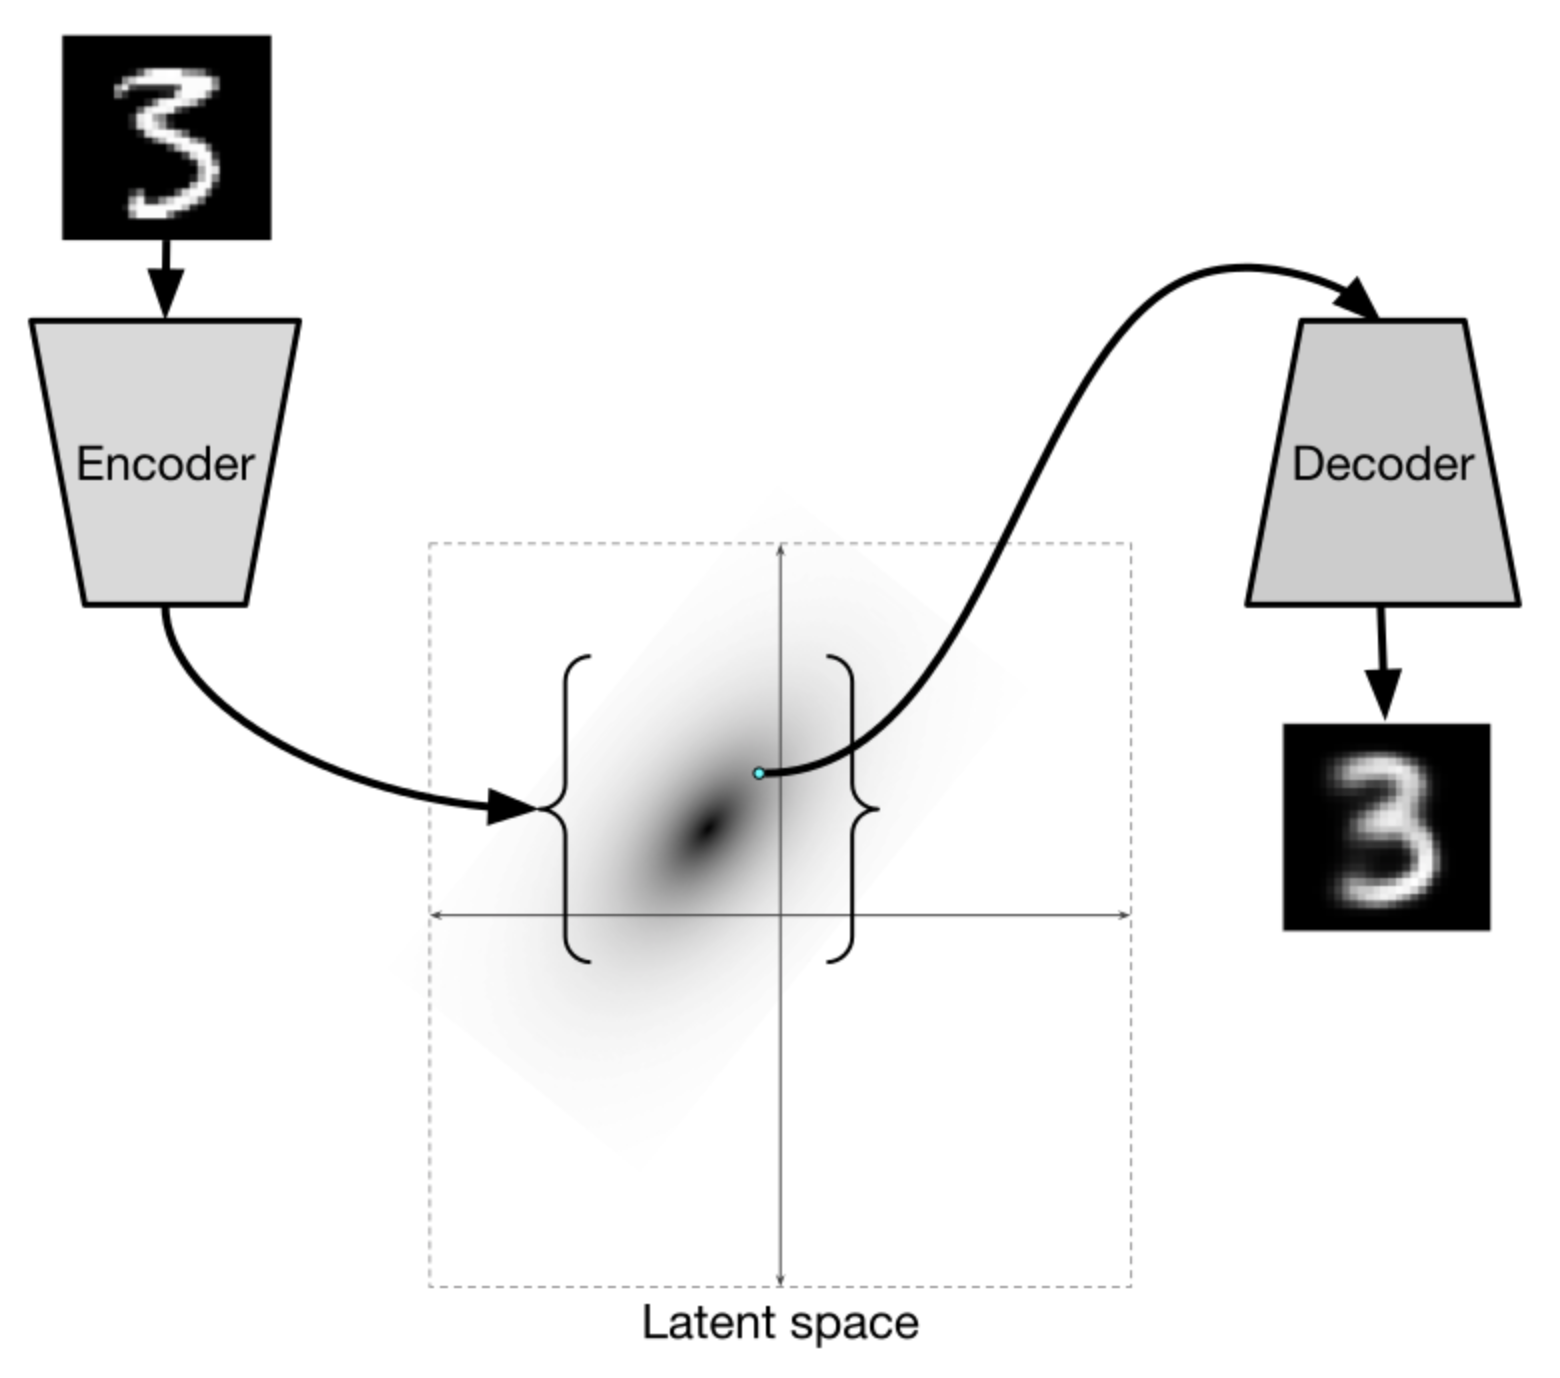
\includegraphics[width=\linewidth]{figs/VAE}
		\end{figure}
	\end{minipage}%
	\begin{minipage}[t]{0.4\columnwidth}
		\begin{figure}[h]
			\centering
			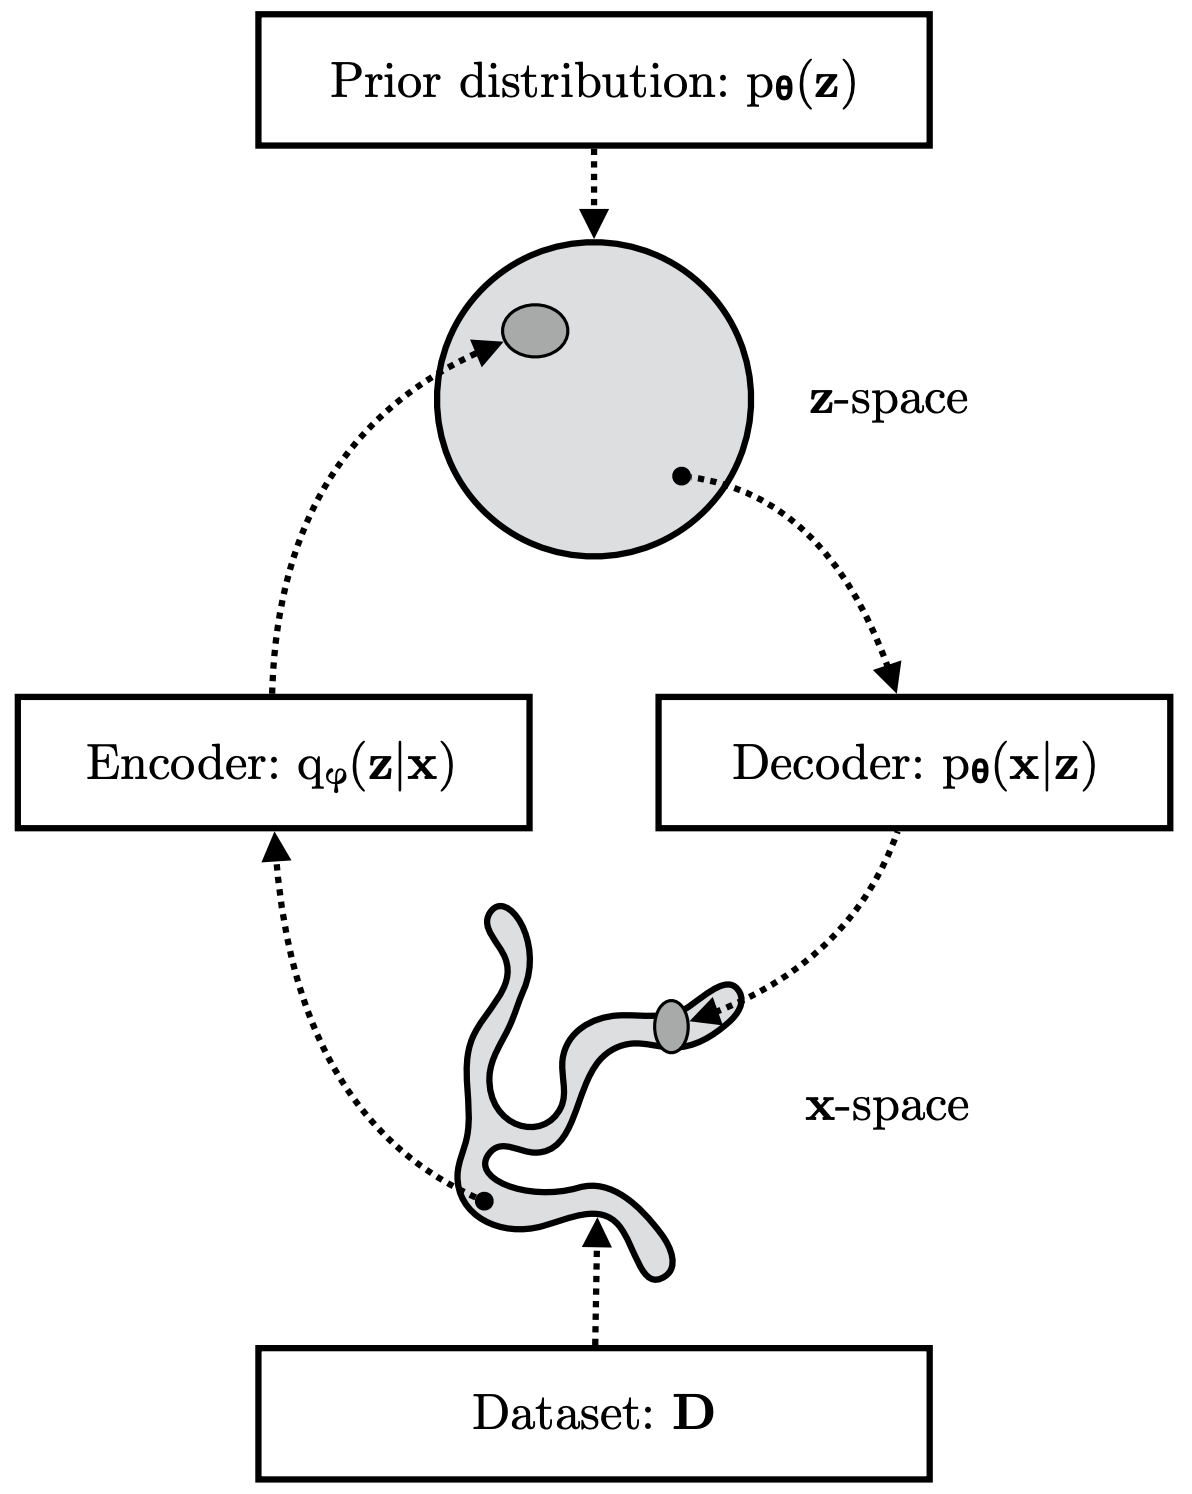
\includegraphics[width=\linewidth]{figs/vae_scheme}
		\end{figure}
	\end{minipage}
	\eqpause
	VAEs are widely used as a preliminary stage of projecting data onto low-dimensional space.
\end{frame}
%=======
\begin{frame}{Variational Autoencoder}
	\myfootnotewithlink{https://arxiv.org/abs/2403.18103}{Chan S., Tutorial on Diffusion Models for Imaging and Vision, 2024}
	\begin{itemize}
		\item The encoder $q_{\bphi}(\bz| \bx) = \text{NN}_{e, \bphi}(\bx)$ outputs $\bmu_{\bphi}(\bx)$ and $\bsigma_{\bphi}(\bx)$.
		\item The decoder $\pt(\bx | \bz) = \text{NN}_{d, \btheta}(\bz)$ outputs parameters of the observed data distribution.
	\end{itemize}
	\begin{figure}[h]
		\centering
		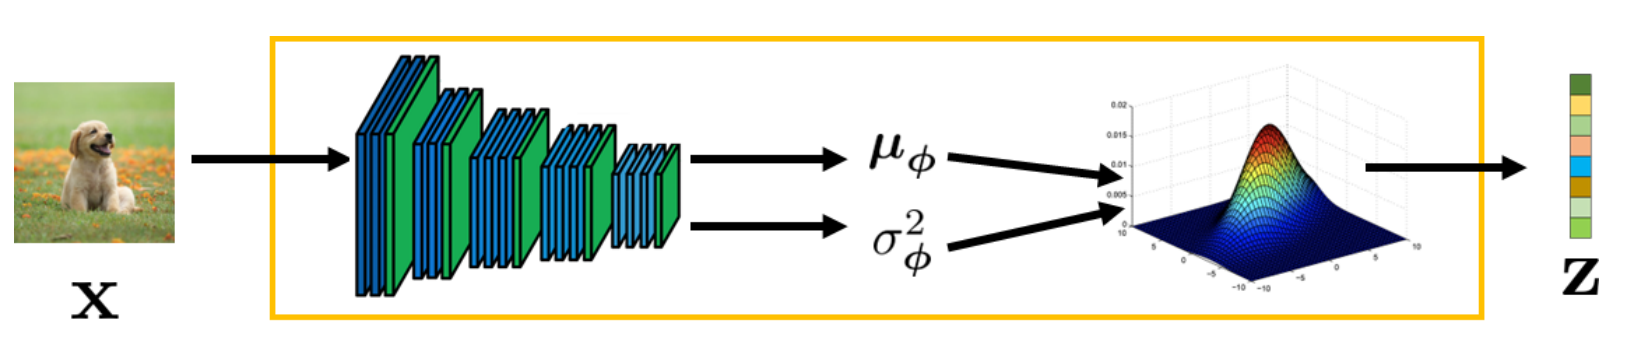
\includegraphics[width=0.7\linewidth]{figs/vae-encoder}
	\end{figure}
	\begin{figure}[h]
		\centering
		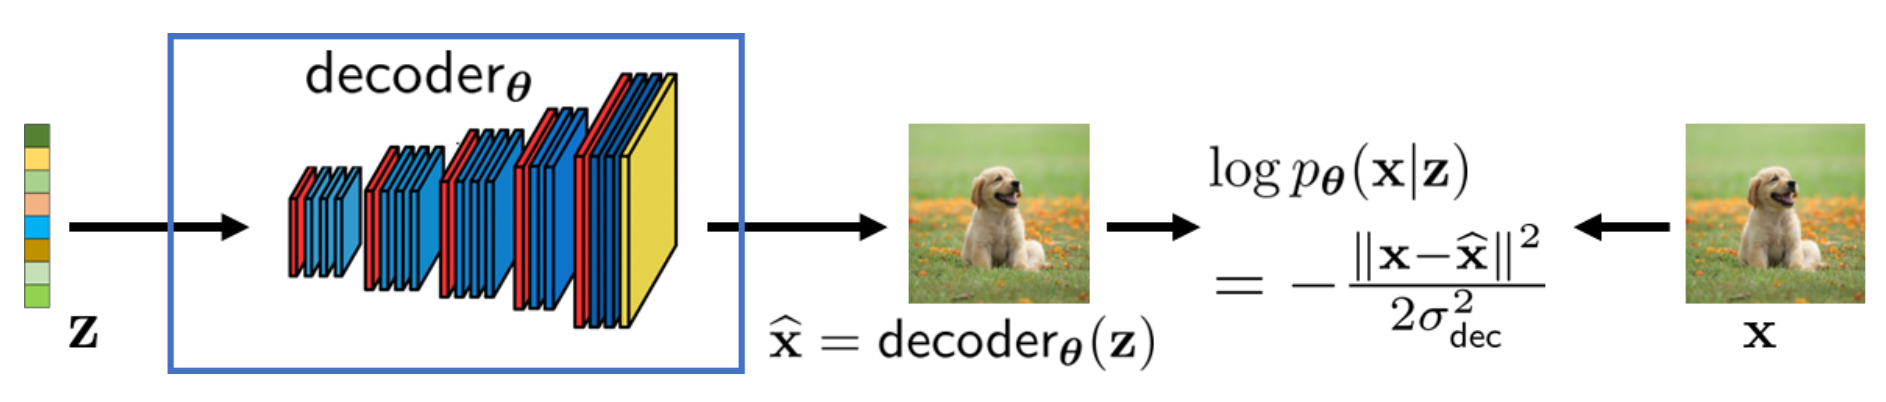
\includegraphics[width=0.9\linewidth]{figs/vae-decoder}
	\end{figure}
\end{frame}
%=======
\begin{frame}{VAE vs Normalizing Flows}
	\myfootnotewithlink{https://arxiv.org/abs/2007.02731}{Nielsen D., et al., SurVAE Flows: Surjections to Bridge the Gap Between VAEs and Flows, 2020}
	\begin{table}[]
		\begin{tabular}{l|c|c}
			& \textbf{VAE} & \textbf{NF} \\ \hline
			\textbf{Objective} & ELBO $\cL$ & Forward KL/MLE \\ \hline
			\textbf{Encoder} & \shortstack{stochastic \\ $\bz \sim q_{\bphi}(\bz| \bx)$} &  \shortstack{\\ deterministic \\ $\bz = \bff_{\btheta}(\bx)$ \\ $q_{\btheta}(\bz| \bx) = \delta(\bz - \bff_{\btheta}(\bx))$}  \\ \hline
			\textbf{Decoder} & \shortstack{stochastic \\ $\bx \sim \pt(\bx| \bz)$} & \shortstack{\\ deterministic \\ $\bx = \bg_{\btheta}(\bz)$ \\ $ \pt(\bx | \bz) = \delta(\bx - \bg_{\btheta}(\bz))$} \\ \hline
			\textbf{Parameters}  & $\bphi, \btheta$ & $\btheta \equiv \bphi$\\ 
		\end{tabular}
	\end{table}
	\vspace{-0.3cm}
	\eqpause
	\begin{block}{Theorem}
		MLE for a normalizing flow is equivalent to maximizing the ELBO for a VAE where:
		\vspace{-0.3cm}
		\[
			\pt(\bx | \bz) = \delta (\bx - \bff^{-1}_{\btheta}(\bz)) = \delta (\bx - \bg_{\btheta}(\bz));
		\]
		\vspace{-0.5cm}
		\[
			q_{\btheta}(\bz| \bx) = \delta (\bz - \bff_{\btheta}(\bx)).
		\]
	\end{block}
\end{frame}
%=======
\begin{frame}{Summary}
	\begin{itemize}
		\item LVMs introduce latent representations for observed data, enabling more interpretable models.
		\vfill
		\item LVMs maximize the variational evidence lower bound (ELBO) to obtain maximum likelihood estimates for the parameters.
		\vfill
		\item Parametric posterior distribution $q_{\bphi}(\bz| \bx)$ makes the method scalable.
		\vfill
		\item The reparametrization trick provides unbiased gradients with respect to the variational posterior $q_{\bphi}(\bz| \bx)$.
		\vfill
		\item The VAE model is a latent variable model parameterized by two neural networks: a stochastic encoder $q_{\bphi}(\bz| \bx)$ and a stochastic decoder $\pt(\bx | \bz)$.
		\vfill
		\item Nowadays, the main role of VAEs is to project data into low-dimensional latent space.
	\end{itemize}
\end{frame}
\end{document}